
\chapter{Background}\label{chap:2}
At first, this chapter presents the growth of malware. Then, malware analysis technique is introduced. Furthermore, malware categories and the way to use Virus total service to identify malware names defined by anti-virus vendor are introduced. Finally, there are problems of using malware name to detect semantic meaning of malware. 
%RELATED WORK
%
%
\section{Growth of malware attack}
Malware can self-replicate recursively. For example, Mota is a kind of worm that proliferate	itself by sending spam email to addresses harvested on local machine \cite{mota}. In addition, Downadup is a malware that receives file through a peer-to-peer function\cite{downadup}. Malware infects system and spreads to the other systems by communication tools such as the Internet and related technologies. 

Since the rise of widespread broadband Internet access, the number of malware samples has been rapidly increasing. According to the report issued by Kaspersky's research team, 205 million pieces of malware were detected and neutralized \cite{kaspersky1}. In addition, in 2010 the number of malware samples increased by 20 millions \cite{kaspersky}.Figure \ref{fig:kaspersky} shows the increase of malware from 2003 to 2009 by Kaspersky Lab. As a result of the fast growth malware, malware is still a huge problem in Internet security and network connectivity. 
\begin{figure}[h!]
\centering
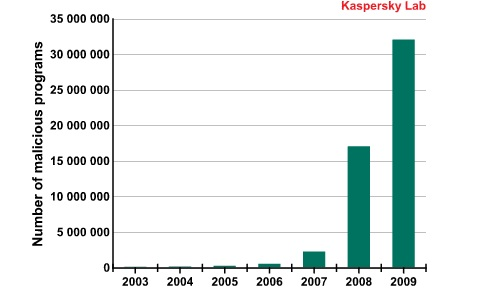
\includegraphics[width=1\textwidth]{graph/kapersky.jpg}
\caption{Number of malicious program}\cite{kaspersky}
\label{fig:kaspersky}
\end{figure}

At this time, malware is easily created by malware creation tools, known the programs which are used by attacker to generate malware\cite{Microsoft}. In addition, unlike early attack tools implementing one type of attack, such tools now can be changed quickly by upgrading or replacing their code. This causes rapidly evolving attacks and, at the extreme, results in polymorphic tools that self-evolve, change with each active instance of the attack. Therefore, a large amount of malware have challenged anti-virus vendor and researcher to avoid their analysis.

\section{Malware avoidance technique}

At the present time, malware is implemented with avoidance technique in order to invalidate static signature based method by anti-virus software and make analysis process more complicated. Avoidance technique can change malware signature and syntax without changing the behaviors of malware. The avoidance technique consists of code obfuscating and packing technique. Therefore, an avoidance technique causes more difficulty in malware analysis. 
 
Obfuscating code changes the form of a malware instance to other form in order to invalidate signature based on detection technique. It consists of polymorphism and metamorphism \cite{blackhat1}. Polymorphic technique modifies the representation of malware. Virus, worm, and other self-propagating software are often used polymorphic technique such as encryption, data appending, and data pre-pending.  Metamorphic malware automatically recodes itself when it distributed or executed\cite{blackhat1}. Simple metamorphic techniques include: adding and varying lengths of NOP instructions, adding useless instruction, and looping the code segment. Advantage metamorphism techniques include: function reordering, program flow modification, static structure modification.

Packing malware can compress the Win32 portable execution file by several tool such as UPX, Winpack, and ExeCryptor. According to a study carried out by Panda Research, $78$\% of new malware used some kinds of file packing to evade detection. PE-packer is designed to reduce the size of malware through compression. The size of packed malware is small but it is bigger when it runs in system\cite{packing}. When uncompressed in memory, packed malware is normally executed. UPX and some PE-packer compress malware binary files and make analysis malware harder.

For the reason that modern malware is implemented with avoidance technique, detection method by the use of static signatures is criticized for being ineffective.   
\section{Malware analysis technique}
This section describes two malware analysis techniques including: dynamic and static analysis. The detail of two techniques is described as follow: 
\subsection{Dynamic malware analysis}
Dynamic malware analysis technique is technique to find out the purpose of malware by running it and making sure what will happen in system. In general, malware is executed in the Virtual Machine. After that, malware researchers use SysAnalyzer, Process Explorer, ProcMon, RegShot, and other tools to identify the general behavioral analysis techniques. For example, SysAnalyser is a useful analysis tool to monitors in many aspects of system and process states such as running process, open ports, loaded drivers, injected libraries, key registry changes, APIs called by a target process, file Modifications, http, IRC, and DNS traffic. Figure \ref{fig:SysAnalyser} shows the example of using SysAnalyser tool to analyse malware. 


\begin{figure}[h!]
\centering
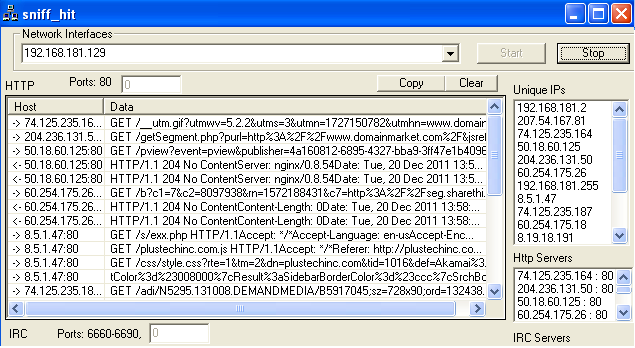
\includegraphics[width=1\textwidth]{graph/SysAnalyser.png}
\caption{SysAnalyser tool for dynamic analysis.}
\label{fig:SysAnalyser}
\end{figure}

The advantage of dynamic malware analysis technique is simple. The process of malware analysis is running malware and making sure what will happen in 
system.

However, there are some disadvantage of dynamic malware analysis technique. At first, these dynamic analysis techniques are vulnerable to a variety of anti-monitoring defenses such as \emph{time bombs} and \emph{logic bombs}. Additionally, these techniques can be slow and tedious to identify and disable. In addition, a dynamic analysis may fail to identify the malware if the behavior of malware is not logged during the analysis process. Furthermore, Much time is required to prepare environment for malware analysis, such as virtual machine environment or sandbox. Moreover, Some malware cannot be executed in virtual machine environment. In conclusion, dynamic technique is not enough for malware analysis. 

\subsection{Static malware analysis}

Static malware analysis is technique that identifies malware program without executing it. With the static malware analysis technique, researcher performs reverse engineering using disassemble tools, decompile tools, source code analyzer tools such as IDA pro and Ollydbg in order to understand malware by seeing the structure of malware. Static malware analysis has an advantage that it can completely discover the purpose and functionality of malware. However, research needs time to understand the malware functionality by analysing malware structure.

In addition, most modern malwares use packer to modify itself. Packer is a program that modify other program files to compress their content. When a packer compress, encrypts, otherwise modifies an executable program, the program looks much different before it was packed. For analysing malware by Ollydbg or IDA pro, malware must be unpacked. PEid is a program that can find the signature of a known compiler or packer. Figure \ref{fig:PEid} shows PEiD is applied to identify identifies the compiler and packer used by the malware author.

\begin{figure}[h!]
\centering
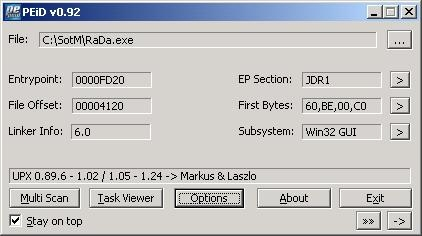
\includegraphics[width=1\textwidth]{graph/PEid.jpg}
\caption{PEid identify the packer used by the malware author.}
\label{fig:PEid}
\end{figure}

Ollydbg is a debugger that shows the assembly instruction of a program as they execute. Breakpoints can be setted on specific instructions to pause execution. Single step through the program one instruction at a time, or let the program run normally. Figure \ref{fig:OllyDbg} show the example of using OllyDbg tool. There are four main windows in Ollydbg debugger: the code window in the center, the register window on the right, the stack window in the bottom right hand  corner and the memory dump window in the bottom left corner. 

\begin{figure}[h!]
\centering
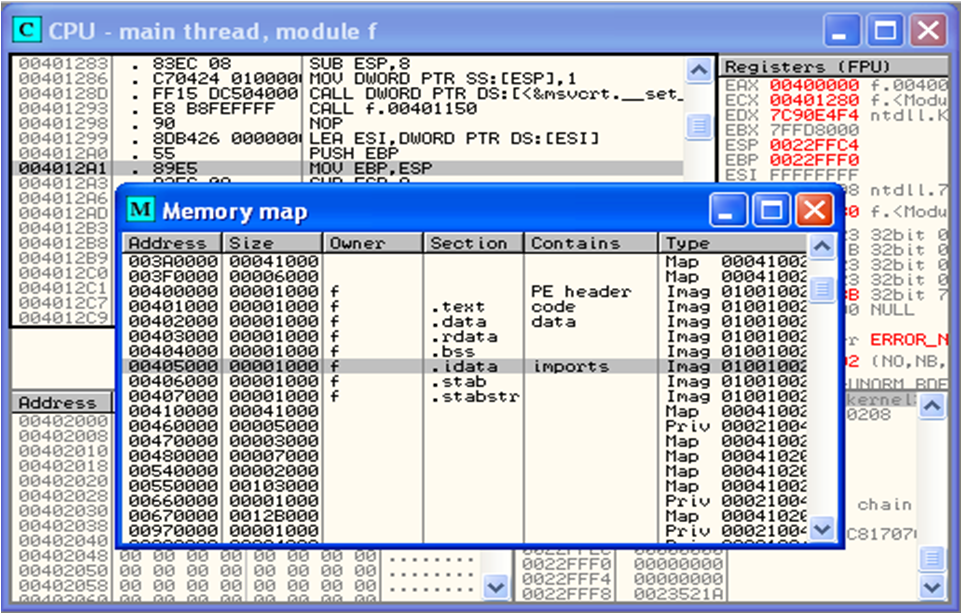
\includegraphics[width=1\textwidth]{graph/OllyDbg.png}
\caption{Ollydbg tool for static analysis.}
\label{fig:OllyDbg}
\end{figure}

IDA pro is a disassembly tool used by many researchers in different areas of reverse engineering. In addition to the disassembly listing, IDA pro also provides control-flow graphs. Figure \ref{fig:IDApro} shows a control-flow graph provided by IDA pro.

\begin{figure}[h!]
\centering
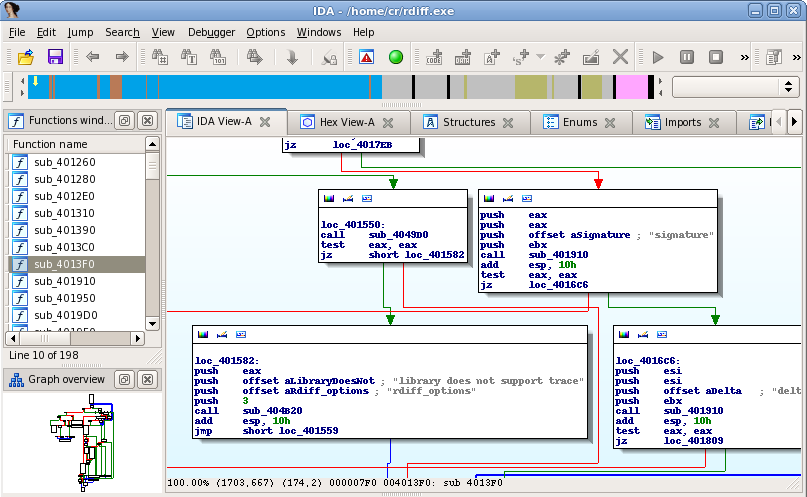
\includegraphics[width=1\textwidth]{graph/idapro.png}
\caption{IDA pro for static analysis.}
\label{fig:IDApro}
\end{figure}


\section{Malware categories}

In general, malware is classified into a few categories or types based on behaviors, method of infection, and the resulting propagation of malware. For example, there are some malware categories: virus, trojan, worm, spyware, and rookit. The categories have specific types of malware threats:

\begin{itemize}
\item Virus :"Software which infects other application and use them as a spreading medium"\cite{BlackHat}.
\item Trojan :"A malicious application which present itself as something else"\cite{BlackHat}.
\item Worm :"Code with ability to spread from computer to computer by means of different network protocols"\cite{BlackHat}.
\item Spyware :"Application aiming to havest personal information"\cite{BlackHat}.
\item Rookit :"Hidden tools providing stealth services to its writer"\cite{BlackHat}.
\end{itemize}

However, the differences between the categories are a bit fuzzy, and the classes are obviously not exclusive. In addition, depending on purpose of virus industry, a unique malware can belong to rookit, virus, or spyware. The detail of malware categories is presented in the next section. 
\subsection{Use virus total to detect the name of categories.}

In this thesis, MD5 hash is used to detect malware name provided by many anti-virus vendor. An MD5 hash is generated by MD5 Message-Digest Algorithm, is a widely used cryptographic hash function that produces a 128-bit (16-byte) hash value. An MD5 hash is typically expressed as a 32-digit hexadecimal number, and MD5 is not collision resistant\cite{wiki1}.

\subsection{Using virus total to getting vendor name}
In this paper, MD5 hash of malware is used to search the name of malware by virus total. Virustotal is a web service that analyzes malware files and facilitates quick detection of viruses, worms, trojans, and all kinds of malware detected by antivirus engines. Malware's name is provided by various anti-virus vendor, but there are many names for unique malware. The Figure \ref{fig:virustotal_listname} reveals malware name detected by antivirus engines. 
\begin{figure}[h!]
\centering
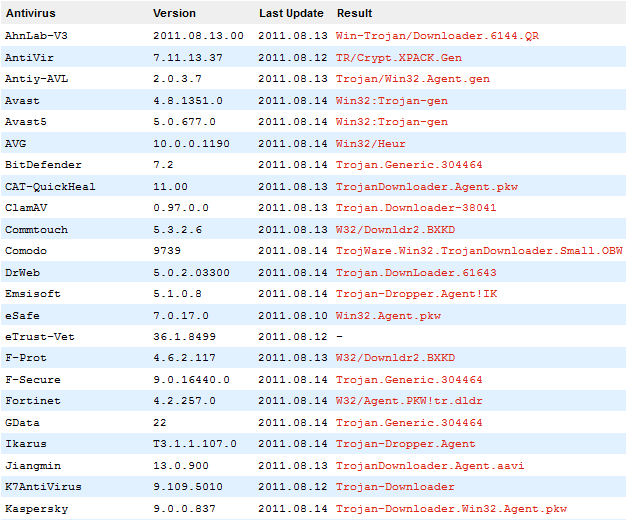
\includegraphics[width=1.0\textwidth]{graph/virustotal_listname.png}
\caption{Malware name is detected by antivirus engines.}
\label{fig:virustotal_listname}
\end{figure}
\section{Problems of malware name} 
As the malware name detected by anti-virus engines is given in Figure \ref{fig:virustotal_listname}, unique malware is not classified into unique name. For each anti-virus vendor, the name of malware detected is different to the other anti-virus vendor. The classification of each anti-virus engine is unlike others. Therefore, malware detected by anti-virus engines cannot provide meaningful characterization of malware for virus researcher. In order to overcome this problem, this paper proposed to classify the malware into families based on malware specific target and its operation behavior. 
As a result of malware name detected by anti-virus vendor was presented above, the new malware families are required for detect meaningful characterization of malware. 
\section{Malware families are used in this paper} 
This paper uses malware families which are reported by Information-technology Promotion Agency \cite{ipa}. The table indicates malware families used in this paper such as Win32/Virut, Win32/Autorun, Win32/IRCbot, Win32/Gaobot, Win32/Waledac, Win32/Downadup, Win32/Sality, and W32.Mota.

\begin{center}
\begin{table}
\begin{tabular}{ l | p{13cm} }
Malware familes & Summary\\ \hline
Win32/Virut & "Win32/Virut is a family of file infecting viruses that target and infect .EXE and .SCR files accessed on infected systems.
 Win32/Virut also opens a backdoor by connecting to an IRC server, allowing a remote attacker to download and run files on the infected computer." \cite{virut}\\ \hline
Win32/Autorun & "Win32/Autorun is a family of worms that spreads by copying itself to the mapped drives of an infected computer. The mapped drives may include network or removable drives." \cite{autorun}\\\hline
Win32/IRCbot & "Win32/IRCbot is a large family of backdoor Trojans that targets computers running Microsoft Windows. The Trojan drops other malicious software and opens a backdoor on the infected computer to connect to IRC servers. The Trojan can maintain multiple IRC server connections simultaneously to receive commands from attackers." \cite{ircbot}\\ \hline
Win32/Gaobot & "The Win32/Gaobot worm family spreads using different methods, depending on the variant. Some variants spread to machines with weak passwords. Others exploit vulnerabilities to infect machines. Once a machine is infected, the worm connects to an IRC server to receive commands." \cite{gaobot}\\ \hline
Win32/Waledac & "Win32/Waledac is a trojan that is used to send spam. It also has the ability to download and execute arbitrary files, harvest email addresses from the local machine, perform denial of service attacks, proxy network traffic and sniff passwords." \cite{walemac}\\ \hline
Win32/Downadup & "Win32/Downadup attempts to spread to network shares by brute-forcing commonly used network passwords and by copying itself to removable drives." \cite{downadup}\\ \hline 
Win32/Sality & "Virus:Win32/Sality is a family of polymorphic file infectors that target Windows executable files with the extensions .SCR or .EXE. They may execute a damaging payload that deletes files with certain extensions and terminates security-related processes and services.\\ \hline 
W32.Mota & W32.Mota is a worm that propagates by sending itself to email addresses gathered from the computer." \cite{mota}\\ \hline 
\end{tabular}
\caption{Malware}
\label{tab:malwarefamilies}
\end{table}
\end{center}

